\chapter{Arquitectura}
\label{cap:arquitectura}



\begin{resumen} 
	
	
\end{resumen}


\section{Buscador de pictogramas}

Ésta herramienta muestra los distintos pictogramas que se asocian a una palabra mediante la API de \textit{ARASAAC}. 

Como se puede ver en la Figura[X] la componente no sólo es un buscador, además tiene un historial de pictogramas añadidos y la opción de preajuste de pictogramas. Dos utilidades muy convenientes de cara a añadir pictogramas al tablero. 

% TODO: \usepackage{graphicx} required
\begin{figure}[h!]
	\centering
	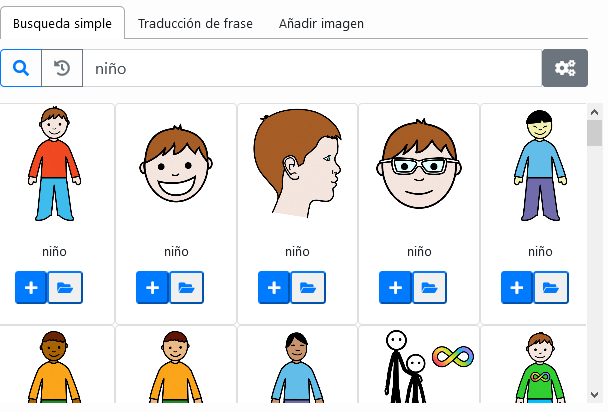
\includegraphics[width=0.7\linewidth]{Imagenes/Bitmap/buscarPicto2}
	\caption{}
	\label{fig:buscarpicto2}
\end{figure}


Para empezar se va a explicar cómo está estructurado el componente de búsqueda de pictogramas. En el estado del componente se almacenará: 

\begin{itemize}
	\item La palabra de la que se quiere obtener sus pictogramas
	\item Los pictogramas encontrados por la consulta
	\item El preajuste de los pictos, donde se especifican cómo se van a mostrar los pictogramas.
	\item Flags de control: Para saber si se ha completado la búsqueda, está abierto el modal o si se ha seleccionado el historial. 	
\end{itemize}


Este componente abarca el acceso a la API, gestión de eventos y los métodos de renderización, en este caso hay dos. El primero que podemos ver en la Figura[1] muestra la barra de búsqueda y sus opciones. El otro método de renderización, muestra el resultado de la consulta, como se puede ver en la Figura[2]. 


% TODO: \usepackage{graphicx} required
\begin{figure}[h!]
	\centering
	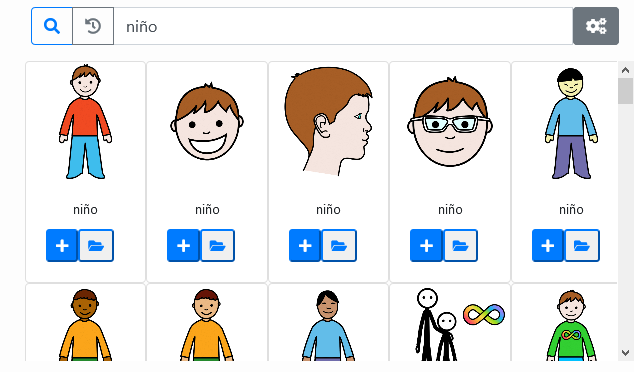
\includegraphics[width=0.7\linewidth]{Imagenes/Bitmap/buscarPicto}
	\caption{}
	\label{fig:buscarpicto}
\end{figure}


A continuación, analizaremos las distintas características de este componente:


\subsection{Búsqueda}

Al pulsar sobre el icono de la lupa o pulsar intro se lanza la consulta a la API mediante Fetch o get. La URL para hacer la petición tiene dos parámetros, el idioma que por defecto es español y el término a buscar. Tras finalizar la búsqueda, se guarda la respuesta de la API para posteriormente procesarla.


Los pictogramas ya buscados, pasan a ser renderizados. Aunque antes de ello es importante explicar el contenido de un pictograma de ARASAAC. De entre todos los parámetros que incluye, destacar: 



\begin{itemize}
	\item \textbf{\_id}: Número único que lo identifica, imprescindible para cargar la imágen.
	
	\item \textbf{Keyword}: La palabra asociada al pictograma.
	
	\item \textbf{hasLocution}: Indica si cuenta con locución. La locución está grabada por una persona y no se trata de una voz robótica típica de un “text to speech”.
	
	\item \textbf{hair}: Indica si el pictograma tiene pelo, en caso afirmativo se puede cambiar su color. 
	
	\item \textbf{skin}: Indica si el pictograma es una persona, en caso afirmativo se podrá cambiar el tono de piel.
		
\end{itemize}

Existen otros muchos parámetros, pero son éstos con los que se han trabajado a lo largo de la aplicación.

En la sección Preajuste se explica en detalle cómo se obtiene y modifica la url. Con la url creada, se mostrarán los pictogramas devueltos por la API. Cada pictograma cuenta con dos botones, uno para añadirlo a la cuadrícula y otro para guardarlo en una lista de pictos. Las listas de pictos se verán en la (Sección de Lista Pictos). 

En caso de añadirlo a la cuadrícula, se guardará en el historial de pictos y enviará la información de éste al componente padre. Éste recibiría el el pictograma que ha devuelto la API de ARASAAC junto a sus parámetros y el preajuste aplicado a dicho picto. Antes de ver el funcionamiento del nuevo ítem que aparecerá en la cuadrícula, es importante conocer el funcionamiento del preajuste e historial.


\subsection{Preajuste}

La manera de obtener la dirección URL de una imagen tiene dos maneras de abordarse. En un primer lugar, podría poner simplemente la url “https://api.arasaac.org/api/pictograms/” junto al identificador del pictograma. De esta manera simplemente se mostraría el pictograma pero perderíamos la valiosa posibilidad de editar un pictograma que ofrece ARASAAC. 

Para poder optar a las modificaciones, se ha de modificar la URL de una manera concreta. Desde la propia API se especifican los atributos modificables que se pueden aplicar a todos los pictogramas:  


\begin{itemize}
	\item \textbf{action}: Añade una flecha para indicar que una acción se da en el futuro o en el pasado.
	\item \textbf{plural}: Añade un “+” en la esquina superior derecha.
	\item \textbf{nocolor}: Muestra el pictograma en blanco y negro.
	 	
\end{itemize}

Existen otras dos modificaciones que solo son aplicables a los pictogramas cuyos parámetros “hair” y “skin” estén marcados como “true“.


\begin{itemize}
	\item \textbf{hair}: Si un pictograma tiene pelo su color puede ser uno de entre 6 colores posibles asociado a su valor hexadecimal. Moreno, rubio, pelirrojo, etc.

	\item \textbf{skin}: Si el pictograma contiene una persona se puede modificar el tono de piel de entre 5 posibles, especificados mediante su valor hexadecimal. 
	
\end{itemize}

Es aquí donde entra en acción el preajuste de pictogramas, ofreciendo al usuario una interfaz donde modificar la apariencia de los pictogramas que se buscan y posteriormente se añadan. Al pulsar sobre el botón [Dónde está] se abre el modal que se ve en la figura [3]. El modal en sí, se trata de otra componente que recibe como parámetro de entrada los preajustes ya establecidos, y devuelve los nuevos preajustes. Los preajustes son los atributos vistos anteriormente: color de pelo, tono de piel, color y plural. 

% TODO: \usepackage{graphicx} required
\begin{figure}[h!]
	\centering
	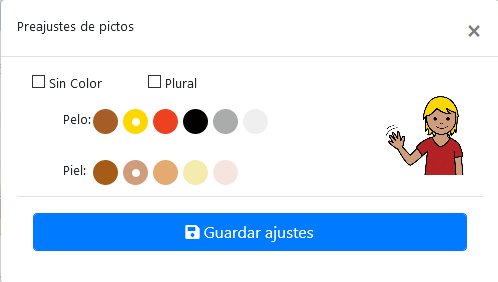
\includegraphics[width=0.7\linewidth]{Imagenes/Bitmap/modalPreajustePicto}
	\caption{}
	\label{fig:modalpreajustepicto}
\end{figure}



La interfaz del modal consiste en dos filas. La primera para los checkbox que marcan las opciones de plural y color, las cuales pueden estar activadas o desactivadas. La segunda fila son para elegir una de entras distintas opciones de color disponibles tanto para el tono de piel como para el color de pelo. 

Está dispuesto de esa manera ya que si se marca algún checkbox, los botones radiales desaparecen. Esto se debe a que no es posible tener por ejemplo, un pictograma sin color y color de pelo rubio. Previniendo así combinaciones que no estén disponibles. 

A la izquierda cuenta con una pre visualización para que el usuario conozca cómo afectan los atributos seleccionados al pictograma. Una vez el usuario esté conforme con los cambios, se envían al componente búsqueda de pictogramas las opciones seleccionadas. 

Respecto a la construcción de las URLs se realiza de la siguiente manera. 

\begin{enumerate}
	\item A partir de la url: https://static.arasaac.org/pictograms/id/id + \{options\} + \_500.png. En la variable \textit{options} se añadirán las opciones que modifiquen el pictograma.
	
	
	\item Dichas opciones deben estar  en un orden concreto utilizando los valores obtenidos del preajuste y el pictograma a crear. Por ejemplo, si se va a crear la url del  pictograma “avion”, los ajustes relacionados con el color de pelo o piel no se aplicarían, ya que el picto no lo permite y por tanto se saltaría.
	
	\item Un resultado posible sería: “\_action-future\_hair-020100\_skin-A65C17” Brevemente, cada etiqueta que se añade significa “\_action-future” que añade la flecha en la esquina superior derecha indicando futuro, “hair” y “skin” van asociados a su color hexadecimal correspondiente obtenido del preajuste. Si la etiqueta de “hair” fuera antes que la de “skin”, la url creada no funciona. De ahí la importancia del orden.
	
	\item La URL creada se usa en el pictograma a mostrar en la interfaz acorde a los preajustes. Como se puede observar en la figura 4, este es el resultado al aplicar los preajustes vistos de la figura 3.
		
\end{enumerate}

% TODO: \usepackage{graphicx} required
\begin{figure}[h!]
	\centering
	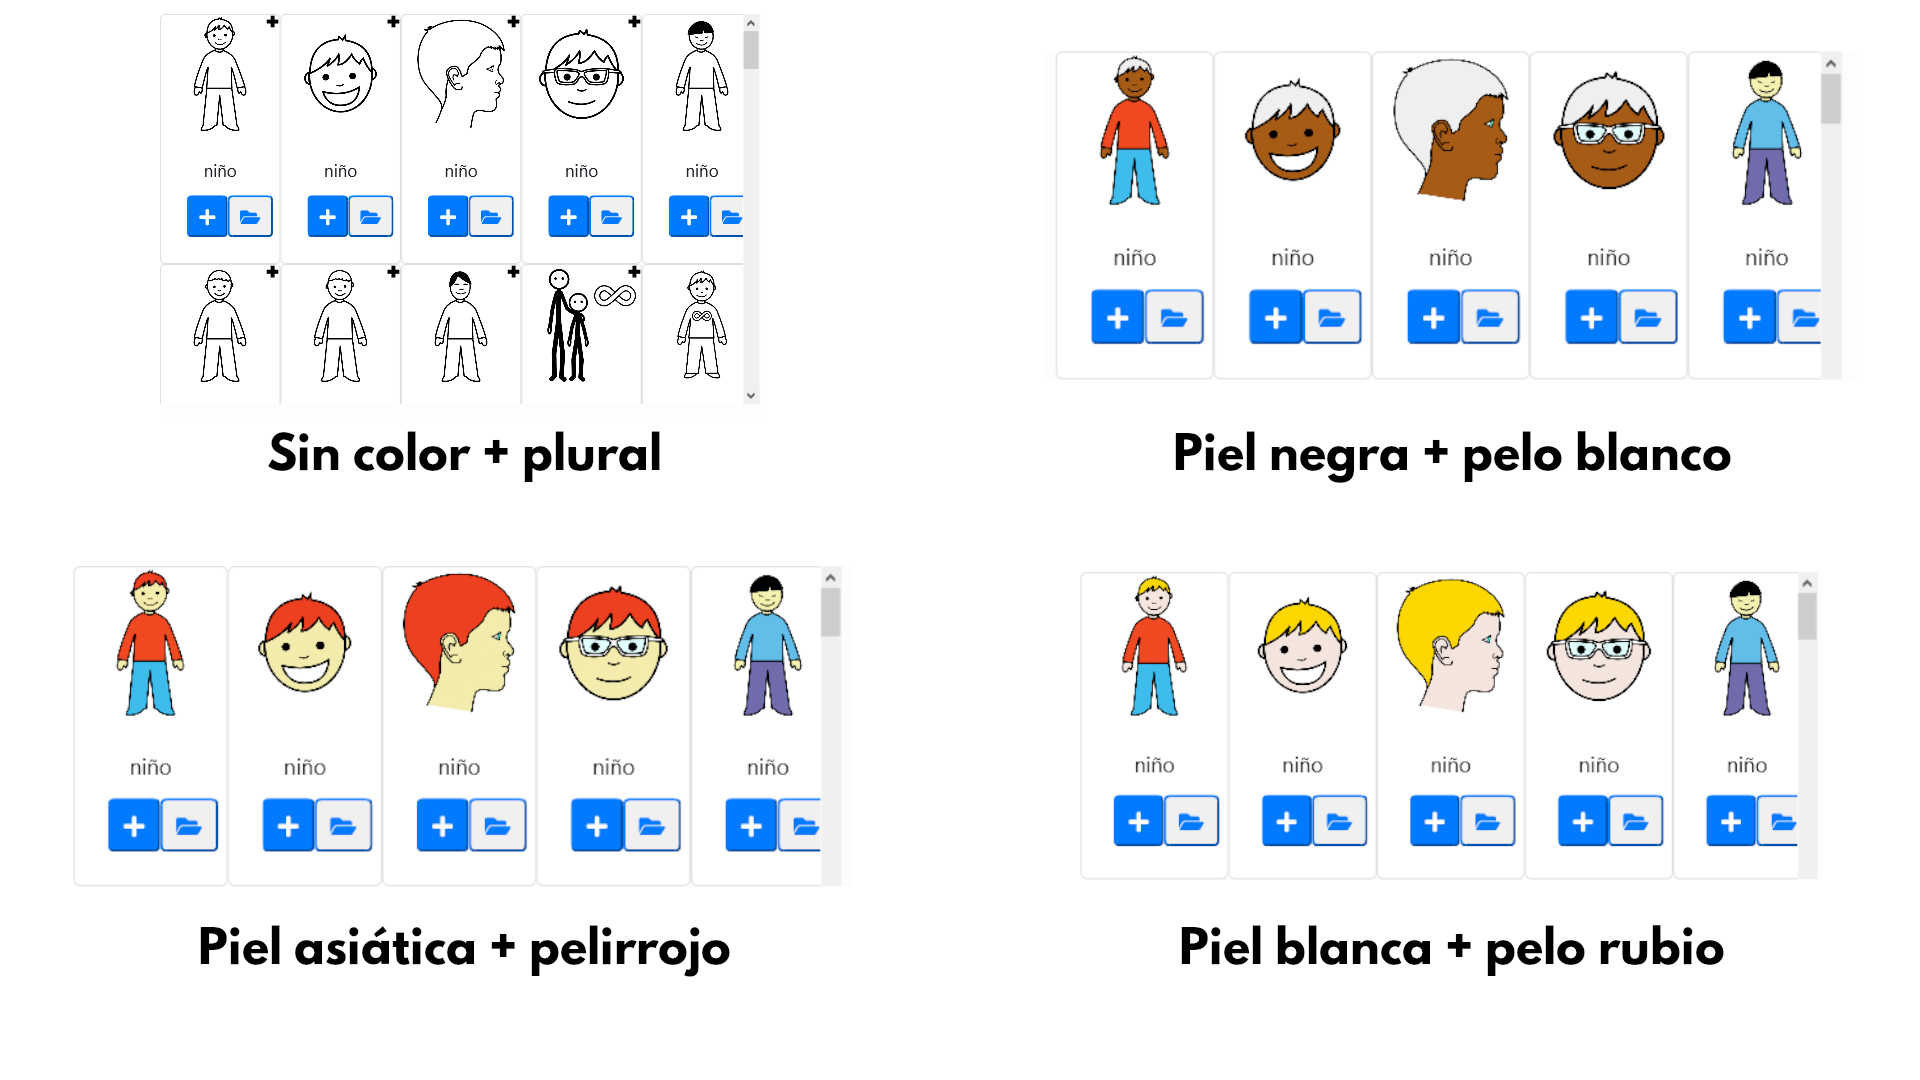
\includegraphics[width=0.7\linewidth]{Imagenes/Bitmap/buscarPictoPreajuste}
	\caption{}
	\label{fig:buscarpictopreajuste}
\end{figure}



\subsection{Historial de pictos}

Al añadir un pictograma al tablero, dicho pictograma se guarda en el historial que se mantiene entre sesiones. Para ello se ha utilizado LocalStorage, el cual almacena una lista en la variable “recentPictos”. Dicha lista está compuesta por el objeto devuelto por la API de ARASAAC parseado a string, ya que los valores almacenados en LocalStorage solo pueden estar en formato UTF-16 DOMString que utiliza dos bytes por carácter. (https://developer.mozilla.org/en-US/docs/Web/API/Window/localStorage) 

Al pulsar sobre el botón de historial  [Figura Historial] se cargarán y mostrarán todos los pictogramas encontrados en “recentPictos”. En caso de haber un historial vacío, se mostrará un mensaje indicándolo. Al igual que la búsqueda, los pictogramas del historial se podrán añadir al tablero o a una lista, y son susceptibles del preajuste de pictogramas.

Es importante destacar que al realizar las pruebas no se puso un límite de pictogramas que se pudieran guardar en el historial. A partir de 300 aparecían pérdidas de rendimiento llegando a detener momentáneamente la página, motivo por el cual se redujo a 50. 


\subsection{PictoItem}

Al añadir el ítem a la cuadrícula, tiene un aspecto similar al de la Figura [5]. Éste ítem ha recibido como parámetros de entrada, el objeto de pictograma devuelto por la API de ARASAAC y el preajuste con el que ha sido añadido. En el caso de la Figura [5], ha sido el pictograma “hola” colocado con preajuste de color de pelo rubio y piel morena. 

% TODO: \usepackage{graphicx} required
\begin{figure}[h!]
	\centering
	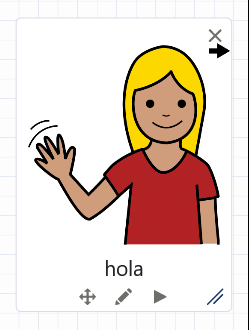
\includegraphics[width=0.7\linewidth]{Imagenes/Bitmap/pictoItemModificado}
	\caption{}
	\label{fig:pictoitemmodificado}
\end{figure}


A continuación se especificarán todas las posibilidades que ofrece un PictoItem colocado en el tablero. 


\section*{Editar Picto}

Tiene un funcionamiento igual al de preajuste de picto aunque se han añadido dos opciones más. Tal y como se puede ver en la Figura [6], éstas son el selector de tiempo verbal y  borde. El motivo de aparición de estas dos opciones en este modal y no en el preajuste es la de no abrumar al usuario. El Borde puede ser de utilidad para los usuarios que quieran resaltar el tipo de pictograma mediante un color, tal y como se vio en capítulos anteriores (Estado de la cuestión). El selector de tiempo verbal sirve para indicar si una acción toma lugar en presente, pasado o futuro.

% TODO: \usepackage{graphicx} required
\begin{figure}[h!]
	\centering
	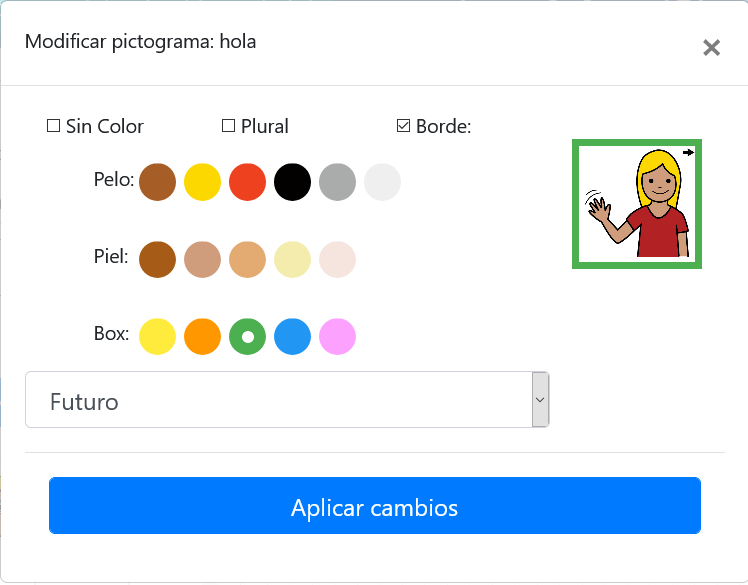
\includegraphics[width=0.7\linewidth]{Imagenes/Bitmap/modalEditarPicto}
	\caption{}
	\label{fig:modaleditarpicto}
\end{figure}


\section*{Reproducir sonido}


La función del botón es la de reproducir mediante audio el nombre del pictograma. Como se ha visto anteriormente, los pictogramas devueltos por la API pueden contar con locución si se consulta el parámetro “hasLocution”. En caso de contar con locución, se accede a la URL que contiene la pista de voz asociada y se reproduce. 
En caso de no contar con locución se ha implementado mediante SpeechSynthesisUtterance para que haga una función similar en el resto de pictogramas. Está configurada para que sintetize la voz en español y es compatible con todos los navegadores modernos.


\section{Traducir frase a pictogramas}

La herramienta de traducción de frase a pictograma, se encuentra en la segunda pestaña que agrupa las herramientas para añadir pictogramas e imágenes. Cuenta con un ítem propio llamado FraseItem, que agrupa los pictogramas de la traducción para ser desplazados con facilidad  por la cuadrícula.

La traducción de frase a pictogramas, como su nombre indica ofrece una interfaz que permite al usuario escribir una frase y recibir la traducción en pictogramas. En la figura [1] se puede ver la interfaz inicial de la traducción a frase, muy similar a la vista en la búsqueda de picto en la figura [1 de los pictos, más arriba]. 

% TODO: \usepackage{graphicx} required
\begin{figure}[h!]
	\centering
	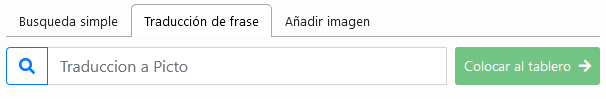
\includegraphics[width=0.7\linewidth]{Imagenes/Bitmap/traducirFraseInicial}
	\caption{}
	\label{fig:traducirfraseinicial}
\end{figure}


La traducción es realizada mediante la API de ARASAAC o NIL Group.


\begin{itemize}
	\item \textbf{API de ARASAAC}: Su API no cuenta con una traducción dedicada a frases, por ello se traduce el texto palabra a palabra de la frase escrita. Por cada palabra devolverá entre 0 o más pictogramas.
	\item \textbf{NIL WS API}:  Cuenta con una función dedicada a la traducción de frases a pictogramas. La traducción resulta mucho más fiel a nivel sintáctico que la planteada  mediante la API de ARASAAC, esto se puede comprobar en la Figura [2]. Las características de NIL WS API será vista en una sección (Sección de NIL Group) más adelante.
\end{itemize}

El resultado de la traducción no está fijado a un pictograma concreto por palabra, sino que puede haber varios. Es por ello que ambas APIs devuelven de un modo u otro varios pictogramas posibles por cada palabra de la frase.  En la Figura [3] se puede ver cómo la interfaz permite navegar entre los pictogramas alternativos mediante dos botones.
Estos botones permiten avanzar y retroceder entre los pictogramas alternativos que se muestran por cada palabra. Por último destacar que el botón “Colocar al tablero” no se activa hasta que no hay una frase traducida, como se puede ver en las figuras [1] y [3]. 

% TODO: \usepackage{graphicx} required
\begin{figure}[h!]
	\centering
	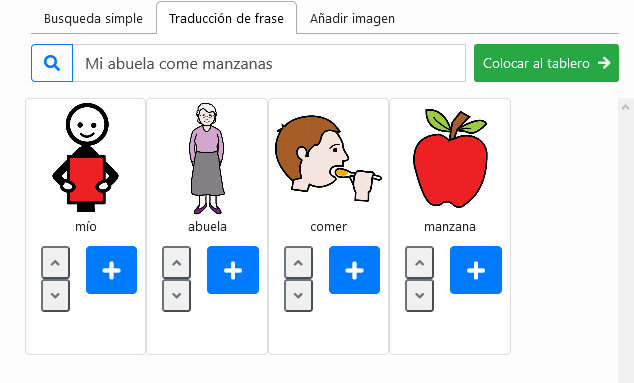
\includegraphics[width=0.7\linewidth]{Imagenes/Bitmap/traduccionPicto}
	\caption{}
	\label{fig:traduccionpicto}
\end{figure}


Antes de añadir la frase a la cuadrícula, es posible añadir los pictogramas en forma individual. En caso que se pulse sobre “Colocar al tablero”, se colocarán en el tablero todos los pictogramas juntos en un único elemento FraseItem. 

\subsection{FraseItem}

Como se puede ver en la Figura [4], el ítem agrupa todos los pictogramas recibidos de la traducción. De esta manera el usuario para desplazarlo por el tablero no tiene que mover cada pictograma de manera individual. Este ítem, cuenta con la posibilidad de ocultar pictogramas ya que el usuario podría no querer que se muestre alguno. Para ello se ha de presionar en el botón de edición con el icono del lápiz. 

% TODO: \usepackage{graphicx} required
\begin{figure}[h!]
	\centering
	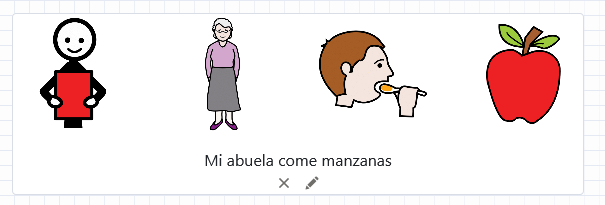
\includegraphics[width=0.7\linewidth]{Imagenes/Bitmap/fraseItemOriginal}
	\caption{}
	\label{fig:fraseitemoriginal}
\end{figure}


Al ser presionado aparecerá un nuevo modal como se ve en la Figura [5. Está compuesto por una previsualización de la frase, los pictogramas que componen la frase junto al botón que permite esconderlo o mostrarlo. Al presionar alguno de ellos, se actualiza la previsualización. En la parte inferior cuenta con un campo de texto para modificar la frase que se muestra en el ítem. En la figura [6] se puede ver un ejemplo de cómo quedaría el ítem tras aplicar los cambios. 

% TODO: \usepackage{graphicx} required
\begin{figure}[h!]
	\centering
	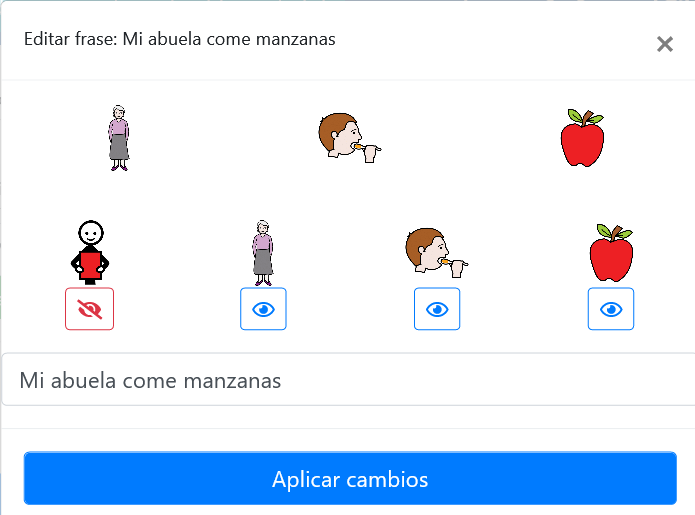
\includegraphics[width=0.7\linewidth]{Imagenes/Bitmap/modalEditarFraseItem}
	\caption{}
	\label{fig:modaleditarfraseitem}
\end{figure}

% TODO: \usepackage{graphicx} required
\begin{figure}[h!]
	\centering
	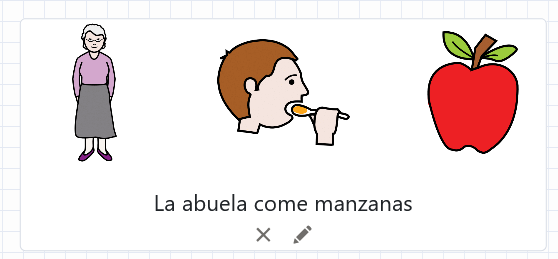
\includegraphics[width=0.7\linewidth]{Imagenes/Bitmap/fraseItemMidificada}
	\caption{}
	\label{fig:fraseitemmidificada}
\end{figure}


\subsection{NIL WS Group}

NIL Word Search es una API que devuelve información relativa a palabras y textos. Respecto al tratamiento de palabras, permite buscar sinónimos, antónimos, emoción, etc. Para el tratamiento de textos, permite  traducir un texto a pictogramas, listar las emociones de un texto o resumir. 

Originalmente la traducción de pictogramas en esta aplicación fue creada específicamente para trabajar con esta API. No obstante también ha causado varios inconvenientes, relativos a los pictogramas que usa la API y los errores causados por CORS. 

La API cuenta con una base de datos propia con una gran cantidad de pictogramas. Pero al traducir un texto a pictogramas. Ésta devuelve por cada palabra o lema, una lista de identificadores. En su mayoría dichos identificadores coinciden con los de los pictogramas de ARASAAC, pero existen otros que no. Estos pictogramas que no comparten identificador con los de ARASAAC por lo que no se puede obtener toda la información deseada, como por ejemplo el texto, audio y modificaciones. Es por ello que PictoItem se modificó para incluir estos pictogramas suprimiendo la posibilidad de personalizar o reproducir el audio.


\subsection{CORS}

Cross Origin Resource Sharing, es un mecanismo de cabeceras http que permite a un servidor dar permiso a otros dominios para cargar recursos del mismo. Por razones de seguridad los navegadores restringen las peticiones de dominio cruzado desde los scripts del navegador. 


Como el proyecto de la web sigue operativo pero descontinuado, no cuenta con la configuración CORS y por tanto no puede recibir peticiones POST de otras webs desde el frontend. Después de comprender el problema se estudió que la solución es crear un backend para la aplicación. Dicho backend está creado exclusivamente para resolver esta petición. El componente de traducción envía la petición al backend, el cual la resolverá gestionando los CORS. En la próxima sección se explicará cómo fue creado. 


Después de crear y configurar el backend de manera local y ver que el componente funcionaba sin complicaciones apareció otro error con la biblioteca html2canvas, encargada de crear una imagen a partir de la cuadrícula y sus ítems. Debido a que las imágenes que retorna la API de NIL son un recurso externo y la biblioteca htm2canvas desconoce su fuente. Por ello al descargar la imagen del tablero estos pictogramas no aparecían representados dejando un hueco en blanco.

\section*{Backend}

El backend fue creado mediante express. Se trata de un framework de Node.js que permite gestionar llamadas a API de manera sencilla. Express cuenta con una dependencia que gestiona los CORS, la cual fue usada para realizar el método post a la API de NIL. 

Para esquematizar cómo se obtienen los pictogramas de la API de NIL, se puede ver en la figura [X] un diagrama de las llamadas que se realizan entre las aplicaciones. 

% TODO: \usepackage{graphicx} required
\begin{figure}[h!]
	\centering
	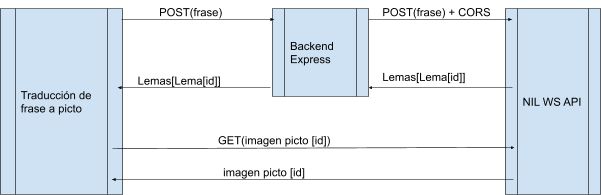
\includegraphics[width=0.7\linewidth]{Imagenes/Bitmap/diagramaConexiones}
	\caption{}
	\label{fig:diagramaconexiones}
\end{figure}


Después de varias semanas investigando todos estos problemas, finalmente se detuvo el desarrollo de este componente ya que la fecha para mostrar la web a los usuarios se acercaba. Al tener un prototipo funcional de traducción mediante API de ARASAAC, asumiendo la baja calidad sintáctica de ésta serviría para estudiar la facilidad de uso de la interfaz por parte de los usuarios.


\section{Añadir imagen al tablero}

Añadir una imagen al tablero se encuentra en la tercera pestaña que agrupa todas las herramientas que añaden pictogramas o fotos a la cuadrícula. Como se puede ver en la Figura [1], su interfaz inicial consiste en un simple botón que carga una imagen del explorador de archivos del dispositivo. Está especificado que solo acepte archivos de tipo imagen, previniendo así posibles errores del usuario. 

% TODO: \usepackage{graphicx} required
\begin{figure}[h!]
	\centering
	\includegraphics[width=0.7\linewidth]{Imagenes/Bitmap/cargarFotoPestaña}
	\caption{}
	\label{fig:cargarfotopestana}
\end{figure}


Al cargar la imagen correctamente, tal y como se puede ver en la FIgura 2 se mostrará: 

\begin{itemize}
	\item Una previsualización de la imagen.
	\item El campo de texto para añadirlo debajo de la imagen.
	\item Botón para añadir la imagen a la cuadrícula.
\end{itemize}

% TODO: \usepackage{graphicx} required
\begin{figure}[h!]
	\centering
	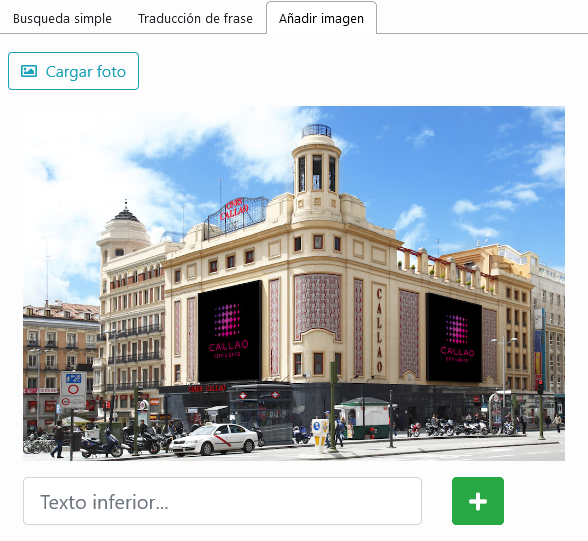
\includegraphics[width=0.7\linewidth]{Imagenes/Bitmap/addPhotoItem}
	\caption{}
	\label{fig:addphotoitem}
\end{figure}



Al presionar el botón de añadir, antes de enviar la información de la foto, se obtiene su valor de alto y ancho en píxeles. Estos datos serán utilizados para conocer la proporción de la imágen. Respecto al valor de la foto seguarda en una URL que funciona únicamente en la sesión vigente mediante  “URL.createObjectURL”.

Al enviar la información de la foto a la capa superior se envían los siguientes parámetros: 

\begin{itemize}
	\item URL de la imagen.
	\item Ancho y alto en píxeles.
	\item Texto inferior, en caso de no haber sido escrito nada se enviará vacío.
\end{itemize}



Al tratar con imágenes y éstas al poder contener material muy sensible, como fotografías personales. Es por este motivo que todos los archivos que pueda cargar el usuario son tratados en el lado del cliente. 

\subsection{PhotoItem}

Su representación en el tablero es la imagen dentro del ítem. El ancho y alto del ítem es proporcional a la imagen original, como se calculó anteriormente. 

Respecto al texto inferior, se puede ver en la Figura 3 puede aparecer o no. Si se ha recibido un texto inferior, éste aparecerá en un espacio reservado para él debajo de la imagen. En caso contrario la imagen abarcará la totalidad del ítem.

% TODO: \usepackage{graphicx} required
\begin{figure}[h!]
	\centering
	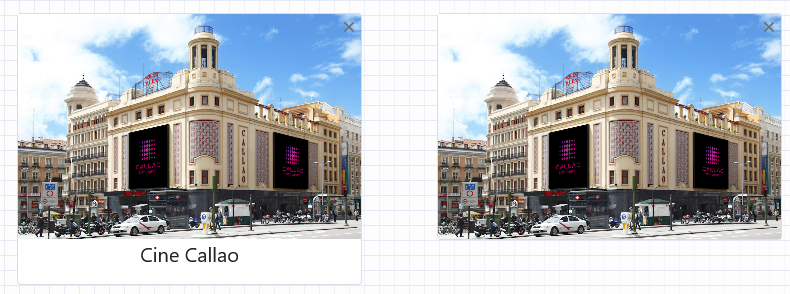
\includegraphics[width=0.7\linewidth]{Imagenes/Bitmap/photoItemTexto}
	\caption{}
	\label{fig:photoitemtexto}
\end{figure}


En la Figura 4 se ejemplifica qué pasaría si en vez de calcular la proporción de la imagen, se dejara siempre con un ancho y alto fijo apareciendo espacios en blanco.

% TODO: \usepackage{graphicx} required
\begin{figure}[h!]
	\centering
	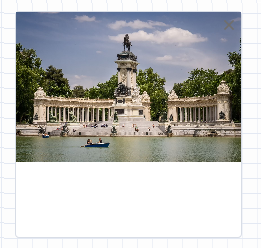
\includegraphics[width=0.7\linewidth]{Imagenes/Bitmap/photoItemError}
	\caption{}
	\label{fig:photoitemerror}
\end{figure}


\subsection{Opciones investigadas y descartadas}

Originalmente hubo dos aproximaciones hacia cómo cargar imágenes. La primera consistía en poder cargar un archivo comprimido zip y mediante la librería JSZip que contaba con funciones para descomprimir archivos. El objetivo era automatizar la colocación de imágenes sobre el tablero, mediante un zip que almacenara éstas junto a un documento con la información de cada una. Dicho documento incluiría el nombre, la posición y el tamaño de cada imagen colocada en la cuadrícula. Descomprimiendo dicho zip, las imágenes volverían a ser colocadas a la posición original.

La otra aproximación ofrecía la posibilidad de conectarse con Google Drive para que el usuario pudiese acceder a sus fotos almacenadas en su cuenta. 

Pese a haber dedicado varias semanas a cada una de estas opciones en proyectos independientes, fueron abandonadas por no obtener resultados satisfactorios. En el caso de JSZip, aunque la compresión de las fotos y descarga del zip funcionara correctamente, surgieron problemas con la librería a la hora de descomprimir los archivos. Respecto a la API de Google Drive, debido a la falta de documentación sobre cómo usarla en React, apenas se logró un prototipo funcional en el tiempo establecido. 

Hubo una última opción que se planteó. Realizar un historial de imágenes cargadas muy similar al historial de pictogramas visto anteriormente. Sin embargo, LocalStorage apenas permitía unos pocos megabytes de almacenamiento. La alternativa a LocalStorage fue indexedDB. 

IndexedDB es una API que permite almacenar información en el cliente, en este caso el ordenador del usuario. En ella se pueden crear bases de datos con la capacidad de almacenar archivos de gran tamaño como en este caso imágenes y fotos. Al final fue descartado por falta de tiempo.





\section{Listas de pictogramas}

Esta herramienta permite crear distintas listas donde el usuario podrá añadir los pictogramas que desee.
Para implementar esta herramienta se necesita tener una estructura donde se guarde el nombre de cada una de las listas y todos los elementos PictoItem que contenga. 

\subsection{Añadir y crear a una lista}

Para poder crear una lista el usuario deberá buscar el pictograma y pulsar el icono de la carpeta del que más le guste. Tras pulsar el icono se desplegará un modal donde dependiendo del estado de las listas mostrará un menú u otro. En el caso de que no haya ninguna lista simplemente se mostrará la opción de crear una lista donde se deberá introducir el nombre de la lista a crear, mientras que si ya había alguna lista creada se mostrará un menú con la posibilidad de añadir el pictograma seleccionado a una lista existente o crear una nueva lista. Un ejemplo de esto lo podemos ver en la Figura [] donde el modal de la izquierda aparece cuando no existe ninguna lista y el de la derecha cuando ya existe al menos una lista. Además la lista mostrada en el modal de la izquierda será la última lista modificada.

% TODO: \usepackage{graphicx} required
\begin{figure}[h!]
	\centering
	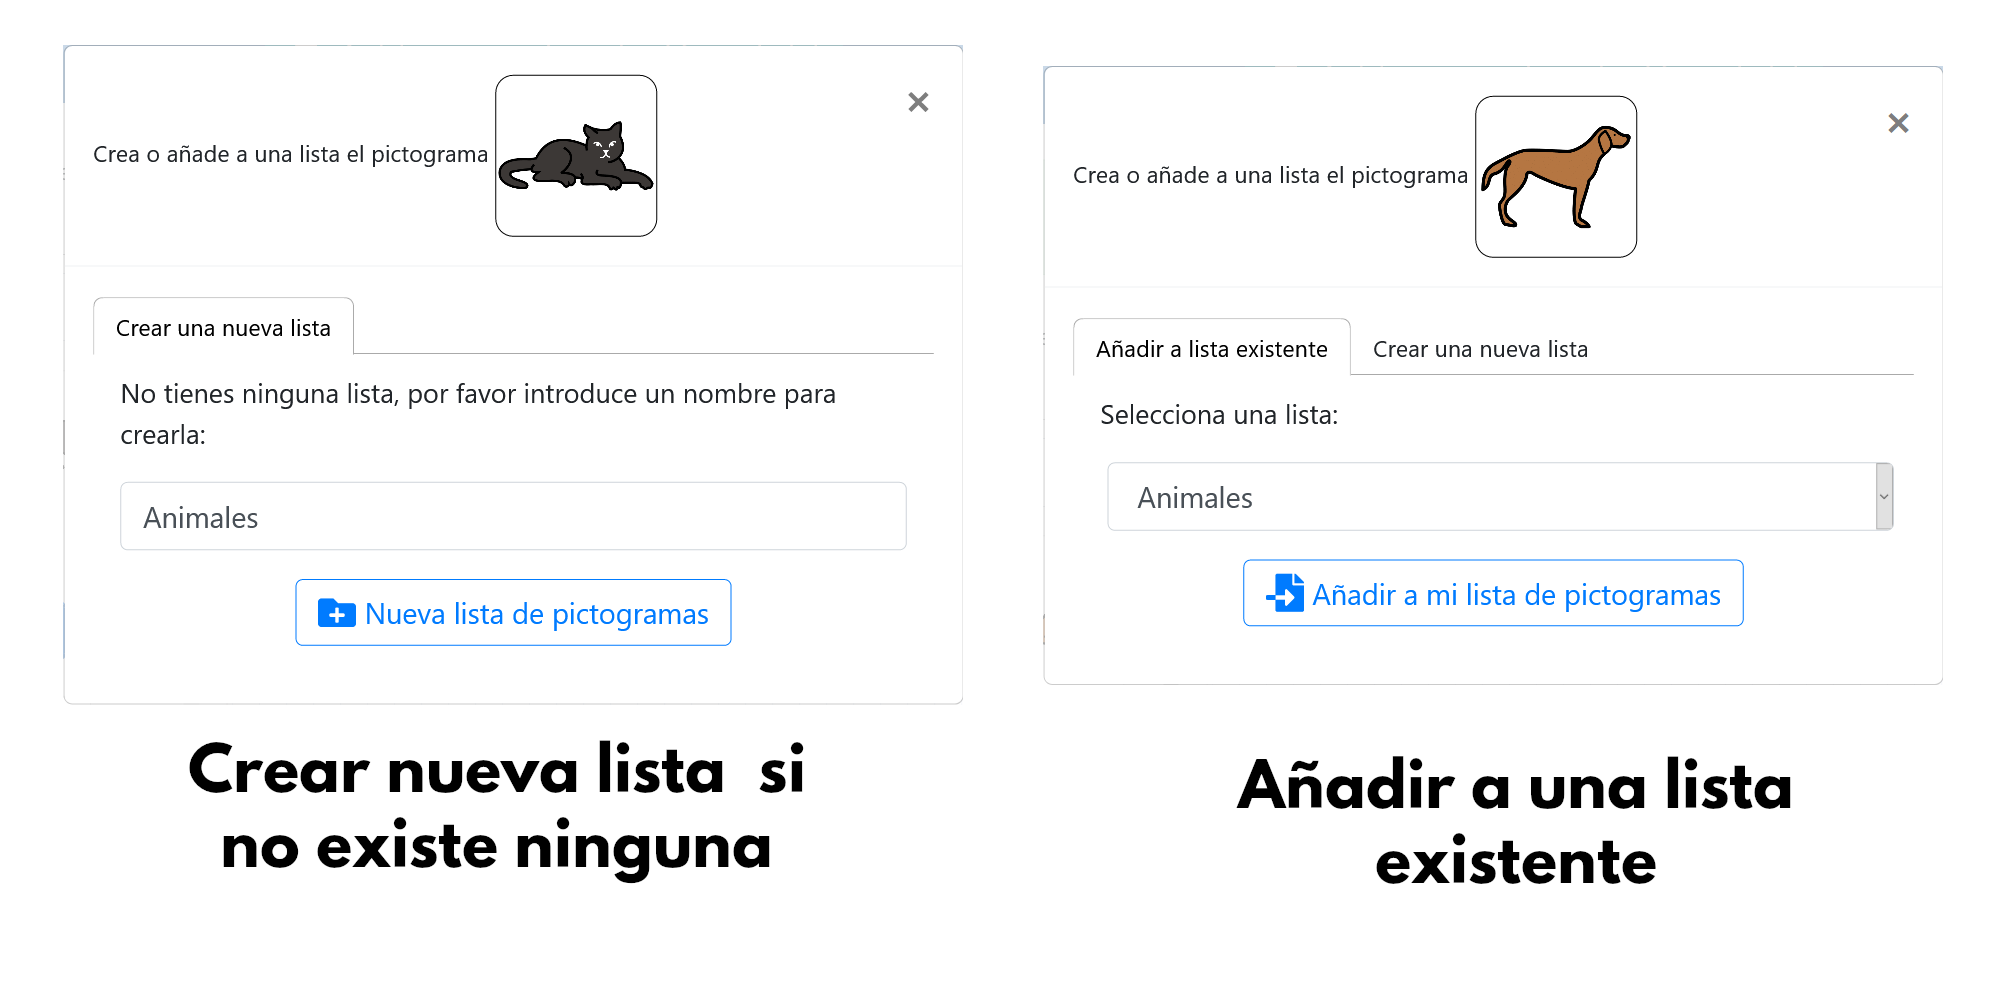
\includegraphics[width=0.7\linewidth]{Imagenes/Bitmap/modalesColeccion}
	\caption{}
	\label{fig:modalescoleccion}
\end{figure}


Para informar al usuario de las acciones tanto la de crear una nueva lista, cómo añadir un pictograma a una lista existente se han utilizado alertas (mensajes). Estas a parte de dar una cierta información al usuario también sirven para tener un cierto control de errores para que el usuario no cree dos listas con el mismo nombre o que no añada un pictograma dos veces a una lista.


\begin{itemize}
	\item En el caso de que se haya podido realizar la acción con éxito se mostrará un pequeño mensaje descriptivo de la acción en verde, ver la figura [].
	
	% TODO: \usepackage{graphicx} required
	\begin{figure}[h!]
		\centering
		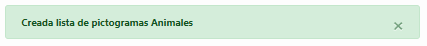
\includegraphics[width=0.7\linewidth]{Imagenes/Bitmap/alertListaPicto}
		\caption{}
		\label{fig:alertlistapicto}
	\end{figure}
	
	
	\item  En el caso de que la acción no se haya podido realizar correctamente se informará al usuario con un mensaje en rojo, como el que se ve en la Figura[], informando al usuario el porqué no ha podido realizarla.
	
	% TODO: \usepackage{graphicx} required
	\begin{figure}[h!]
		\centering
		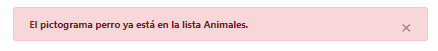
\includegraphics[width=0.7\linewidth]{Imagenes/Bitmap/alertErrorListaPicto}
		\caption{}
		\label{fig:alerterrorlistapicto}
	\end{figure}
	
	
	
\end{itemize}

\subsection{Listas de Pictogramas creadas}

Otras funcionalidades que podemos encontrar en esta herramienta es la posibilidad de importar y exportar las listas creadas.
Para la funcionalidad de exportar guardaremos el estado actual de las listas en un fichero con extensión “.json”. Para la generación de este documento se utilizará la función \textit{JSON.stringify()}, la cual nos permitirá crear la estructura propia de los json y posteriormente generar el documento con ese contenido.

La funcionalidad de importar cargará el estado de las listas a partir del archivo creado anteriormente. Para ello se hará uso de la función \textit{JSON.parse()} la cual convertirá el json a la estructura de listas requerida. En caso de ya existir listas en la aplicación, las nuevas listas cargadas se añadirán a las ya existentes. 

Por último, las listas existentes se encuentran en el apartado “Mis listas de pictogramas”, como se muestra en la figura []. Para visualizar una de ellas deberemos seleccionar el nombre de esta de entre todas las disponibles. A continuación, al igual que en el apartado de búsqueda de pictograma, se mostrarán todos los pictogramas con su imagen, texto correspondiente y el botón de “+” que permite añadirlo a la cuadrícula como un PictoItem visto anteriormente.

% TODO: \usepackage{graphicx} required
\begin{figure}[h!]
	\centering
	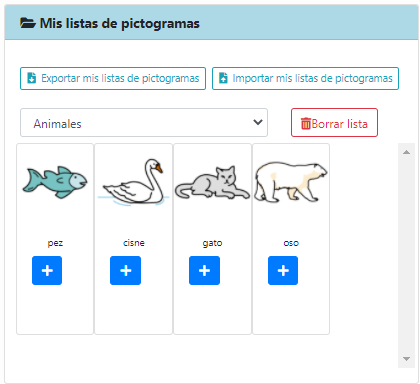
\includegraphics[width=0.7\linewidth]{Imagenes/Bitmap/lisaPictoSel}
	\caption{}
	\label{fig:lisapictosel}
\end{figure}


\section{Texto}

Esta herramienta permite añadir un cuadro de texto a la cuadrícula. Como opciones de personalización de texto se ofrece la posibilidad al usuario de seleccionar una tipografía entre las seis posibles. Las tipografías elegidas son las más utilizadas dentro del ámbito educativo.

Esta herramienta se puede encontrar en el apartado de “Personalización de tablero”, donde se podrán seleccionar distintas tipografías y escribir el texto que se va a añadir a la cuadrícula.

Como se puede ver en la Figura [X] en la parte superior se puede elegir una tipografía y a su derecha ver una previsualización de ésta. Debajo, está el campo de texto donde se escribirá la frase seguido del botón para añadirla a la cuadrícula.

% TODO: \usepackage{graphicx} required
\begin{figure}[h!]
	\centering
	\includegraphics[width=0.7\linewidth]{Imagenes/Bitmap/añadirTexto}
	\caption{}
	\label{fig:anadirtexto}
\end{figure}


Para poder implementar este componente, en su estructura se guardará el texto que se vaya a añadir a la cuadrícula y la tipografía seleccionada.

A diferencia de otros elementos como los pictogramas en los que el ancho y alto del ítem era proporcional, en el texto se permite ajustar ambas propiedades de manera independiente.

\subsection{TextoItem}

Al añadir el texto a la cuadrícula, el ancho del ítem se ajustará al número de caracteres del texto. En la parte inferior del ítem como se ve en la Figura [X] se encuentran tres botones, dos para reducir y aumentar el tamaño de la fuente del texto y otro para editar su contenido.

% TODO: \usepackage{graphicx} required
\begin{figure}[h!]
	\centering
	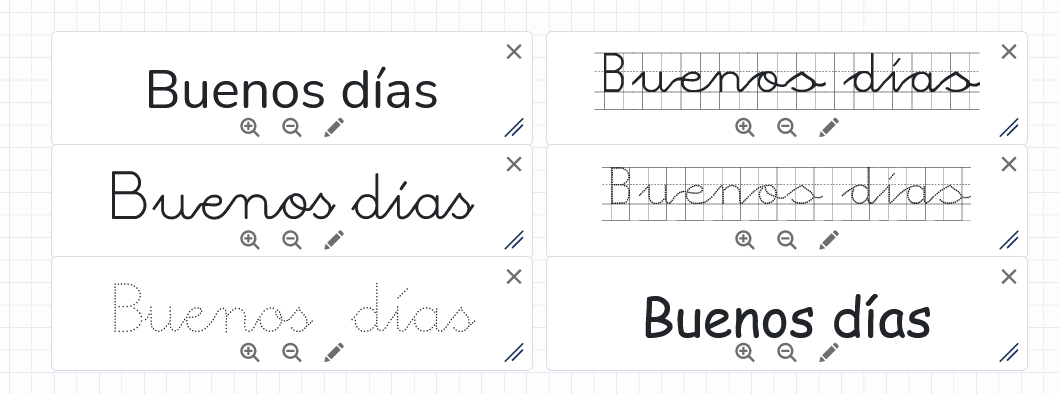
\includegraphics[width=0.7\linewidth]{Imagenes/Bitmap/fraseItem1}
	\caption{}
	\label{fig:fraseitem1}
\end{figure}


Al pulsar sobre el icono del lápiz se desplegará el modal de edición de ítem. Como se ve en la imagen [X] cuenta con un campo donde se puede ver y editar el contenido actual del texto. Esto resultará muy útil para corregir errores ortográficos. Tras pulsar sobre el botón “Cambiar texto”, el ancho del ítem se ajustará de nuevo en función del nuevo número de caracteres.

% TODO: \usepackage{graphicx} required
\begin{figure}[h!]
	\centering
	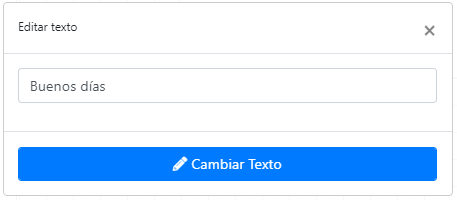
\includegraphics[width=0.7\linewidth]{Imagenes/Bitmap/modalEditarTexto}
	\caption{}
	\label{fig:modaleditartexto}
\end{figure}



\section{Iconos}

La componente iconos permite añadir a la cuadrícula iconos y personalizarlos. Los iconos disponibles son: cuadrado, tick, barra y corazón, como se muestra en la figura [1]. La componente está formada por una estructura donde se guarda el tipo de icono, el color y la opacidad. Al ser añadidos a la cuadrícula tiene un color por defecto en función del tipo de icono, verde para el tick y rojo para la barra y el corazón.

% TODO: \usepackage{graphicx} required
\begin{figure}[h!]
	\centering
	
\includegraphics[width=0.7\linewidth]{Imagenes/Bitmap/herramientaItems}
	\caption{}
	\label{fig:herramientaitems}
\end{figure}


A la hora de mostrar los iconos en la cuadrícula hay que hacer una distinción entre el cuadrado y el resto de los iconos ya que la forma en la que se muestran es distinta.

Para generar un cuadrado se hace uso de las formas geométricas básicas que ya están implementadas en SVG. Este lenguaje de marcas permite crear figuras geométricas y personalizar su aspecto. Para representar el cuadrado se ha de incluir la etiqueta \textit{<rect/>} (etiqueta para generar un cuadrado) y añadir las propiedades que queremos que tenga como por ejemplo altura, ancho, grosor de los bordes del cuadrado, color u opacidad.

Sin embargo, para el resto de los iconos se utiliza Font Awesome. Este framework tiene implementado iconos vectoriales que al igual que con el cuadrado, permiten la personalización de los iconos respecto a el color, tamaño y opacidad. Para mostrarlos se deberá incluir la clase correspondiente de cada icono especificada en el apartado tipo de la estructura.

En la figura [] se puede ver que estos iconos se pueden superponer a los pictogramas para realzar ideas.

% TODO: \usepackage{graphicx} required
\begin{figure}[h!]
	\centering
	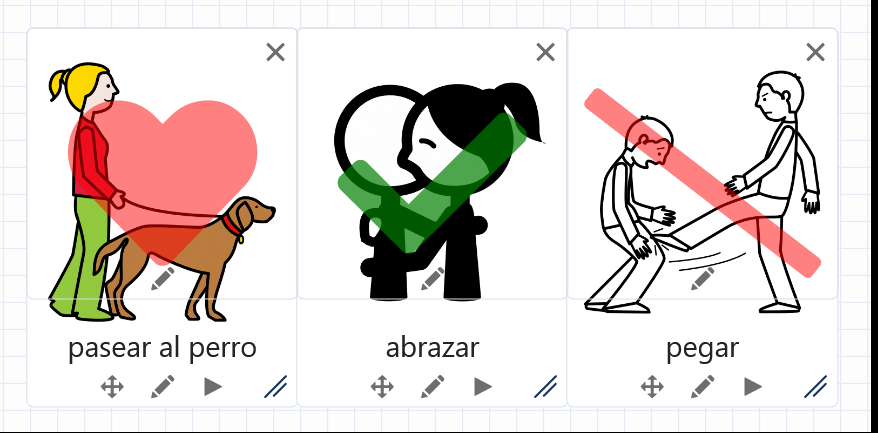
\includegraphics[width=0.7\linewidth]{Imagenes/Bitmap/ejemploPictoItem}
	\caption{}
	\label{fig:ejemplopictoitem}
\end{figure}

 
Aunque la forma de visualizarlos se hace de manera distinta dependiendo del icono todos ellos permiten editar ciertos aspectos, es por ello por lo que se incluyó la funcionalidad de editar. Para poder editar un icono añadido a la cuadrícula tendremos que pulsar sobre el icono del lápiz, al pulsarlo aparecerá un modal, como el de la Figura [] donde se podrá modificar el color y la opacidad de la figura.  

% TODO: \usepackage{graphicx} required
\begin{figure}[h!]
	\centering
	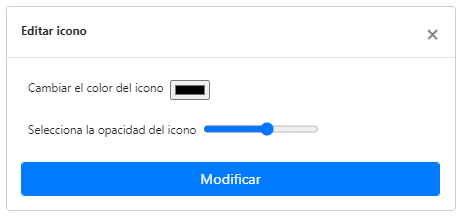
\includegraphics[width=0.7\linewidth]{Imagenes/Bitmap/modalPictoItem}
	\caption{}
	\label{fig:modalpictoitem}
\end{figure}


\section{Descargar Tablero}


Esta herramienta permite descargar la cuadrícula como imagen. Para ello se utiliza la librería html2tocanvas. Ésta librería además permite seleccionar la calidad de descarga de la imagen. Por ello que se ha creado un modal como se puede ver en la Figura [X] donde el usuario puede elegir la calidad deseada, siendo la calidad alta la elegida por defecto. 


% TODO: \usepackage{graphicx} required
\begin{figure}[h!]
	\centering
	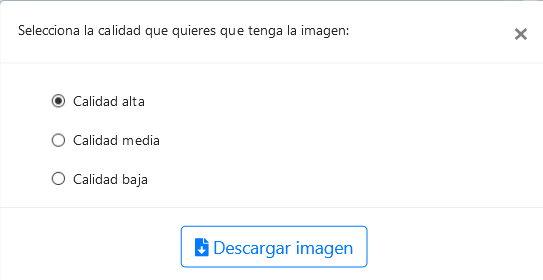
\includegraphics[width=0.7\linewidth]{Imagenes/Bitmap/modalDescargarTablero}
	\caption{}
	\label{fig:modaldescargartablero}
\end{figure}




